\documentclass[a4paper,11pt]{article}
\usepackage[latin1]{inputenc}
\usepackage[T1]{fontenc}
\usepackage{bbm}
\usepackage{amsmath}
\usepackage{indentfirst}
\usepackage{fullpage}
\usepackage{url}
\usepackage{graphicx}
\usepackage[center,footnotesize]{caption}
\usepackage[section]{placeins}
\usepackage{subfig}
\usepackage{booktabs}
\usepackage{color}
\providecommand{\e}[1]{\ensuremath{\times 10^{#1}}}

\title{Genomics and Bioinformatics}
\author{Exam solutions}
\begin{document}
\maketitle

\section*{Question 1}

\begin{enumerate}
\item %includegraphics[height=0.2\textwidth]{exam_graph_fig0.pdf}
AATGCATGCAATGCGA
\item 
\begin{eqnarray*}
S_4 &=& \{\mbox{AATG, ATGC, TGCA, GCAT, CATG, GCAA, CAAT, TGCG, GCGA}\}.\\
  S_5&=&\{\mbox{AATGC, ATGCA, TGCAT,} \\
  &&\phantom\{\mbox{GCATG, CATGC, ATGCA,} \\
  &&\phantom\{\mbox{TGCAA, GCAAT, CAATG,} \\
  &&\phantom\{\mbox{AATGC, ATGCG, TGCGA}\}.
\end{eqnarray*}
\item \phantom{XXXX}
\begin{figure}[h]
\centering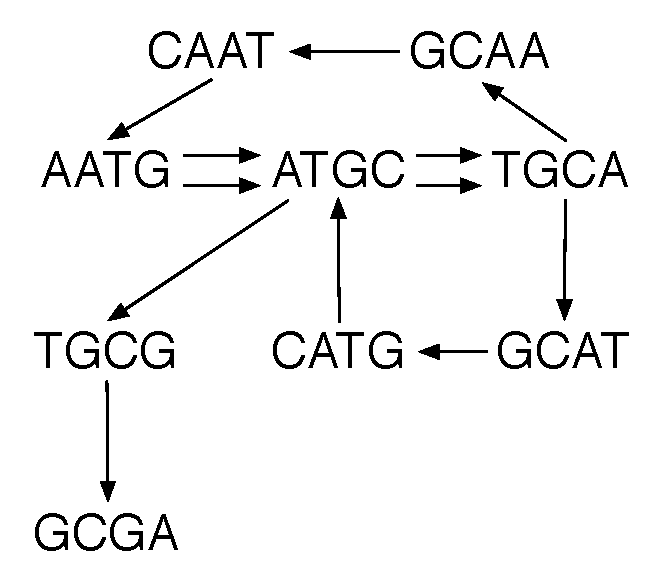
\includegraphics[scale=.5]{exam_graph_fig1.pdf}
\end{figure}
\item 
Possible paths are\\\\
\small{AATG-ATGC-TGCA-GCAT-CATG-ATGC-TGCA-GCAA-CAAT-AATG-ATGC-TGCG-GCGA}\\
\small{AATG-ATGC-TGCA-GCAA-CAAT-AATG-ATGC-TGCA-GCAT-CATG-ATGC-TGCG-GCGA}\\\\
\normalsize{leading to two possible maximum length contigs}:\\\\
AATGCATGCAATGCGA\\
AATGCAATGCATGCGA
\begin{figure}[h]
\centering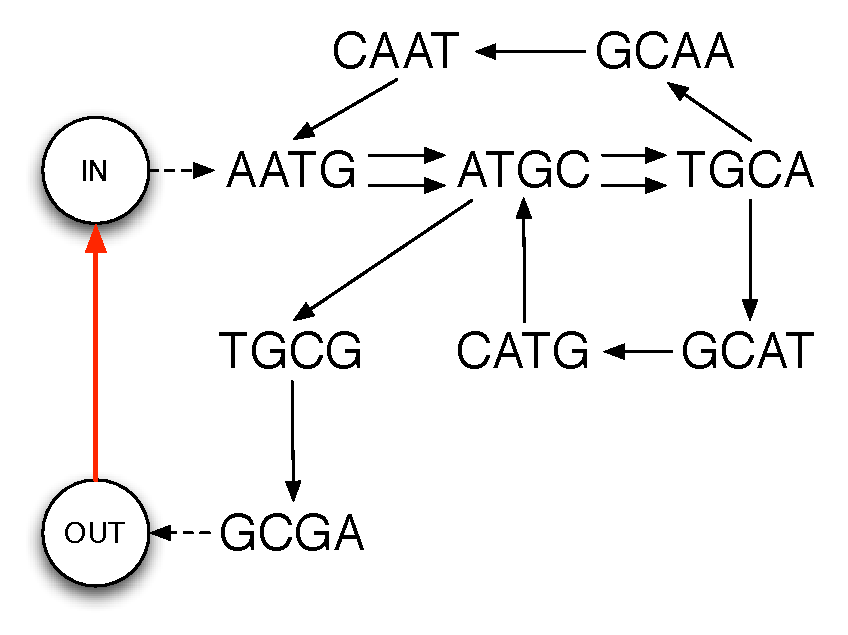
\includegraphics[scale=0.5]{exam_graph_fig2.pdf}
\end{figure}
\end{enumerate}

\section*{Question 2}
\subsection*{Sequence alignment}
\begin{verbatim}
ACGTATAGGC
AC-TA-A-GC
\end{verbatim}
\begin{table}[ht]
  \begin{center}
    \begin{tabular}{rccccccccccc}
      \toprule
      & - & A & C & G & T & A & T & A & G & G & C\\
      \midrule
      - & $0$ & $-2$ & $-4$ & $-6$ & $-8$ & $-10$ & $-12$ & $-14$ & $-16$ & $-18$ & $-20$\\
      A & $-2$ & \colorbox{red}{1} & $-1$ & $-3$ & $-5$ & $-7$ & $-9$ & $-11$ & $-13$ & $-15$ & $-17$\\
      C & $-4$ & -1 & \colorbox{red}{2} & \colorbox{red}{0} & $-2$ & $-4$ & $-6$ & $-8$ & $-10$ & $-12$ & $-14$\\
      T & $-6$ & -3 & 0 & 1 & \colorbox{red}{1} & $-1$ & $-3$ & $-5$ & $-7$ & $-9$ & $-11$\\
      A & $-8$ & -5 & -2 & -1 & 0 & \colorbox{red}{2} & \colorbox{red}{0} & $-2$ & $-4$ & $-6$ & $-8$\\
      A & $-10$ & -7 & -4 & -3 & -2 & 1 & 1 & \colorbox{red}{1} & \colorbox{red}{-1} & $-3$ & $-5$\\
      G & $-12$ & -9 & -6 & -3 & -4 & -1 & 0 & 0 & 2 & \colorbox{red}{0} & $-2$\\
      C & $-14$ & -11 & -8 & -5 & -4 & -3 & -2 & -1 & 0 & 1 & \colorbox{red}{1}\\
      \bottomrule
    \end{tabular}
  \end{center}
\end{table}

\subsection*{Modified gap penalty}

This above alignment has $7$ matches, $3$ gaps and $3$ gap
openings. The score is therefore
$$
7\times 1-3\times 1-3\times 2\,=\,-1~.
$$

Below is another alignment:
\begin{verbatim}
ACGTATAGGC
AC---TAAGC
\end{verbatim}
It has $6$ matches, $1$ mismatch, $3$ gaps and 1 gap opening and a
score of:
$$
6\times 1-1\times 1-3\times 1-1\times 2\,=\,0~.
$$

\section*{Question 3}

\begin{eqnarray*}
\mathcal{M}&=&\bordermatrix{
    &I_0&M_1&I_1&M_2&I_2&M_3&I_3&\cr
 I_0&0.2&0.8&0  &0  &0  &0  &0  \cr
 M_1&0  &0  &0.2&0.8&0  &0  &0  \cr
 I_1&0  &0  &0.2&0.8&0  &0  &0  \cr
 M_2&0  &0  &0  &0  &0.2&0.8&0  \cr
 I_2&0  &0  &0  &0  &0.2&0.8&0  \cr
 M_3&0  &0  &0  &0  &0  &0  &1\cr
 I_3&0  &0  &0  &0  &0  &0  &1}~,\\
\mathcal{E}&=&\bordermatrix{
&I_0&M_1&I_1&M_2&I_2&M_3&I_3&\cr
A&0.25&0.6&0.25&0.2&0.25&0  &0.25\cr
C&0.25&0  &0.25&0.8&0.25&0.4&0.25\cr
G&0.25&0  &0.25&0  &0.25&0  &0.25\cr
T&0.25&0.4&0.25&0  &0.25&0.6&0.25}~,
\end{eqnarray*}

\begin{figure}[h]
\centering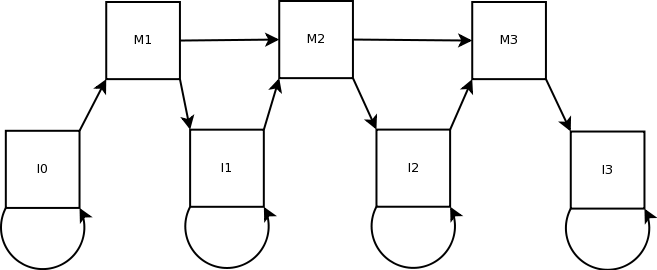
\includegraphics[scale=.5]{HMM.png}
\end{figure}

\begin{table}[ht]
  \begin{center}
    \begin{tabular}{rccccccccccc}
      \toprule
      & - & G & A & C & A & T \\
      \midrule
      $I_0$&$1$&$\colorbox{red}{5/4}$&$25/16$&$125/64$&$625/256$&$3125/1024$\\
      $M_1$&$0$&$0  $&$\colorbox{red}{15}$&$0     $&$375/16 $&$625/32   $\\
      $I_1$&$0$&$0  $&$0    $&$75/4  $&$375/16 $&$1875/32  $\\
      $M_2$&$0$&$0  $&$0    $&$\colorbox{red}{240}$&$75     $&$0        $\\
      $I_2$&$0$&$0  $&$0    $&$0     $&$\colorbox{red}{300}$&$375      $\\
      $M_3$&$0$&$0  $&$0    $&$0     $&$0      $&$ \colorbox{red}{3600}$\\
      $I_3$&$0$&$0  $&$0    $&$0     $&$0      $&$0        $\\
      \bottomrule
    \end{tabular}
  \end{center}
\end{table}

The corresponding multiple alignment is:
\begin{verbatim}
-AC-T
-AA-T
-AC-C
-TC-T
-TC-C
GACAT
\end{verbatim}


\section*{Question 4}

\begin{enumerate}
\item 
\begin{center}
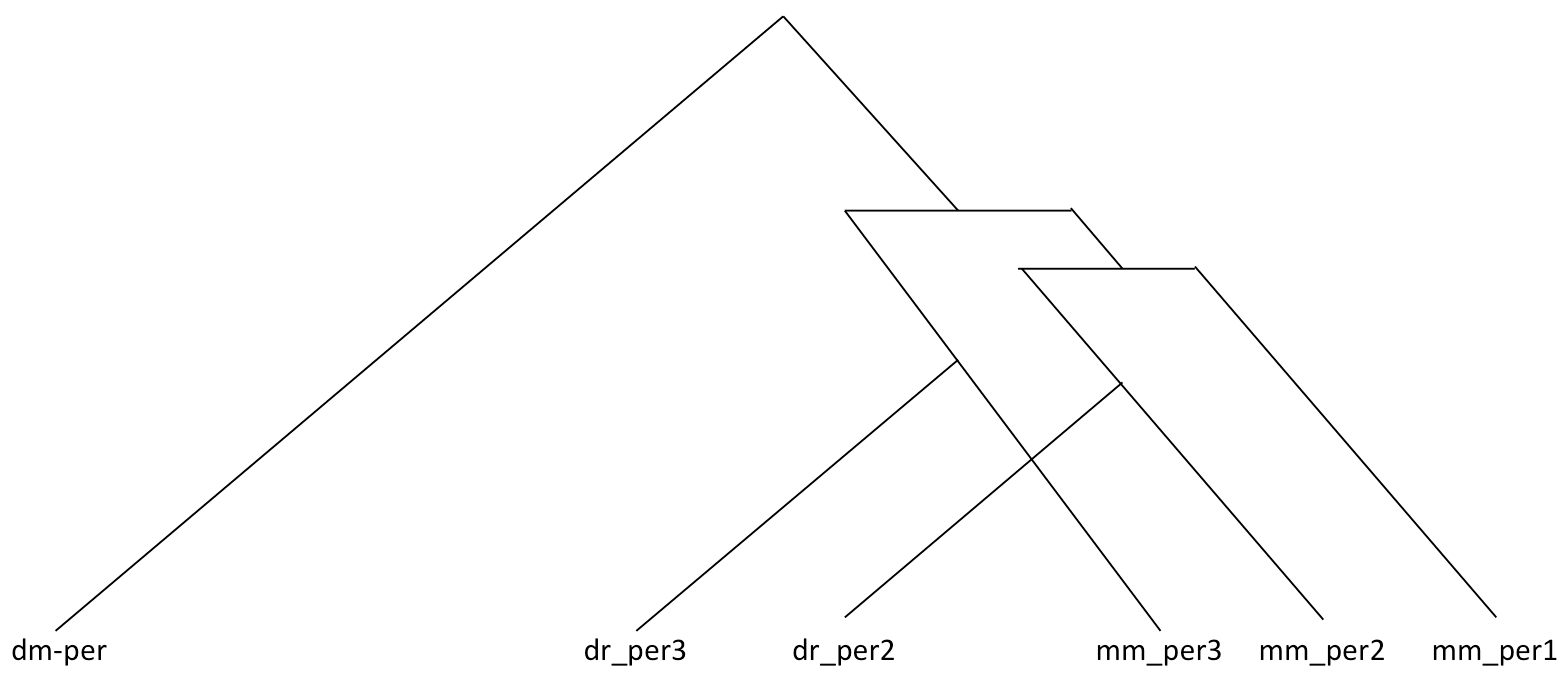
\includegraphics[width=0.8\textwidth]{tree.png}\\
\vspace{0.5cm}
{\bf The gene tree}
\end{center}

\item
\begin{itemize} 
\item An orthologous pair: {\bf dr\_per2} and {\bf mm\_per2}

\item A paralogous pair in the same species: {\bf mm\_per1} and {\bf mm\_per2}

\item A paralogous pair in different species: {\bf mm\_per1} and {\bf dr\_per2}
\end{itemize}
\end{enumerate}

\end{document}
